\documentclass[11pt]{article}
\usepackage{icmlko}
\begin{document}

\title{죽은 것은 모듈이 아니라 내 대본이었다 --- 노트 415 정정과, 그제야 잰 값}
\author{월드모델 실험실}
\date{노트 416 · 2026년 8월 2일}
\maketitle

\begin{abstract}
\textbf{노트 415를 정정한다.} 거기서 \texttt{popaxes} 의 축 넷이 ``노트 358
이후로 죽어 있었다''고 적었다. \textbf{틀렸다.} 죽은 것은 모듈이 아니라
\textbf{내 시험 대본}이다.

\texttt{\_idol} 은 \texttt{make\_extra} 가 \textbf{호출 가능}이면
\texttt{set\_grades} 를 건 \emph{뒤에} 부른다. 나는 extras 를 \textbf{미리
조립한 딕트}로 넘겼고, 그러면 \texttt{popaxes.build()} 가 GRADES$=$(A,B)
일 때 실행돼 \textbf{75행}이 나온다 --- 판의 팝업은 89행이라 길이 불일치로
버려진다. 호출 가능으로 넘기면 \textbf{89행}에 관측 표시자 $0.85 \sim 0.88$
이다.

\textbf{노트 359가 이미 이 자리를 적어 뒀다} --- \emph{같은 거름망이 두 군데
적혀 있으면 갈라진다}(그 노트가 세어 ``여덟 번째''라 했다). 노트 359는 그
갈라짐을 고치려고 \texttt{set\_grades} 를 만들었다. \textbf{나는 그것을 안
쓰는 경로로 부르고는 모듈이 고장 났다고 적었다.}

그래서 사전 등록 ③(\emph{단일 도메인 축은 판에 해롭다} --- 노트 413의 규칙)이
노트 415에서 \textbf{시험되지 않았다}. 제대로 다시 걸었다.

\begin{center}
\begin{tabular}{lrr}
\hline
짝 12뽑기, $+$popaxes & 차 & 부호 \\
\hline
\textbf{판} & $\mathbf{-0.0003}$ & $\mathbf{2/12}$ \\
\textbf{팝업} (축을 받은 도메인) & $\mathbf{-0.0033}$ & $4/12$ \\
시장팝업 & $-0.0059$ & $2/12$ \\
\hline
\end{tabular}
\end{center}

\textbf{사전 등록 ③ 통과.} 그리고 규칙보다 한 걸음 더 나갔다 --- 노트 412의
\texttt{mkt} 는 적어도 \emph{제 도메인}은 $+0.0241$ 로 벌었는데,
\texttt{popaxes} 는 \textbf{제 도메인도 못 번다}($-0.0033$).
\end{abstract}

\section{넓은 축만 판에 온다}

이번 사이클에 판에 올린 축 넷을 한자리에 놓으면 규칙이 선명하다.

\begin{center}
\begin{tabular}{lrrl}
\hline
축 & 덮는 도메인 & 판 차 & 결과 \\
\hline
\texttt{grp} & 8 & $+0.0029 \cdot 11/12$ & \textbf{채택}(노트 413) \\
\texttt{seq} & 7 & $-0.0000 \cdot 7/12$ & 애니엔 $+0.0103$, 도서가 지움 \\
\texttt{mkt} & \textbf{1} & $+0.0005 \cdot 6/12$ & 제 도메인 $+0.0241$ \\
\texttt{pop} & \textbf{1} & $-0.0003 \cdot 2/12$ & \textbf{제 도메인도 $-0.0033$} \\
\hline
\end{tabular}
\end{center}

한 도메인만 아는 열은 두 번 다 판에 못 왔다. 노트 413이 적은 대로
\textbf{그런 열은 자질이 아니라 도메인 이름표를 한 번 더 적는 것}이고,
표시자 무늬가 이미 도메인을 유일하게 부르는 마당에(노트 404: 열한 중 아홉이
순도 $1.000$) 이름표는 남아돈다.

\section{가드는 제 일을 했다}

노트 415에서 만든 \texttt{\_dead\_axes} --- \emph{표시자가 어디서도 1 이
아닌 축을 실행 기록에 남긴다} --- 는 \textbf{내 잘못된 빌드를 즉시 짚었다.}
진단이 틀렸을 뿐 관측은 맞았다: 그 빌드에서 그 네 열은 정말로 아무 값도
안 날랐다.

가드를 남긴다. 다만 주석을 고쳤다 --- 원인은 ``모듈이 옛 행 수로 지어졌다''가
아니라 \textbf{``extras 를 언제 조립했느냐''}다. \textbf{둘 다 관문에서는
``무해''로 보인다}는 것이 이 가드의 존재 이유다.

\section{남은 것}

\begin{tabular}{lp{7.2cm}}
\hline
시장팝업 $+0.0241$ & 노트 412의 값은 여전히 갈 곳이 없다. 단일 도메인 축
둘 중 \textbf{하나는 값이 있고 하나는 없다} --- 그 차이가 다음 갈래 \\
extras 조립 시점 & 이 경로로 지어진 다른 축이 더 있나. \texttt{\_dead\_axes}
가 이제 매 실행에 찍는다 \\
도서 & 학습 80행으로 축 추가마다 판정을 뒤집는다(노트 415) \\
\hline
\end{tabular}

\begin{figure}[h]
\centering
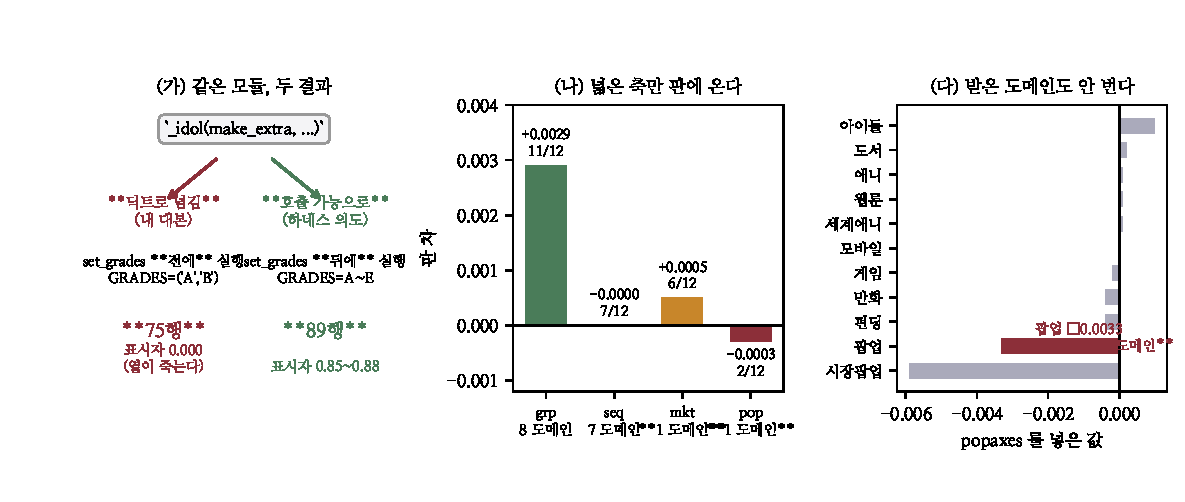
\includegraphics[width=\textwidth]{figs/fig416.pdf}
\caption{(가) 같은 모듈이 조립 시점에 따라 75행 · 89행으로 갈린다.
(나) 덮는 도메인이 넓은 축만 판에 온다. (다) \texttt{popaxes} 는 축을 받은
팝업조차 못 벌게 한다.}
\end{figure}

\end{document}
